% Project structure
%!TEX root = ../Project.tex
\section{Project Structure \& Specification}
\label{sec:project_structure___specification}

This appendix contains all the technical information of the `project' and the data format used.

\begin{figure}[htbp]
	\centering
		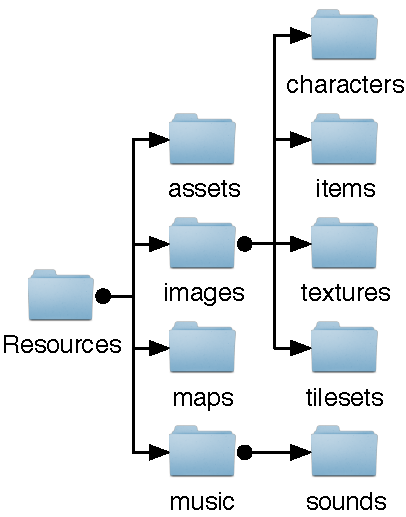
\includegraphics[height=3in]{figures/Files.pdf}
	\caption{Project Structure}
	\label{fig:figures_Files}
\end{figure}

A game's resources  are organised as shown above. One of the main restrictions, is that all external links have to be relative to the \texttt{resources} directory. All \texttt{xml} files \textbf{must} conform to the schemas in the \texttt{schemas} directory. 


\subsection{Assets}
Assets are stored in the following format:
\begin{lst:resource}[caption=Assets format]
<name>
  <entry>
    <uuid>128bit</uuid> 
    <resource uuid="128 bit">
    </resource>
  </entry>
</name>
\end{lst:resource}

The \texttt{assets} directory \textbf{must} contains the following files conforming to schemas in \texttt{schemas/assets}.
\begin{lstlisting}[caption=Required Assets]
maps.xml
music.xml
ordering.xml
skills.xml
sounds.xml
textures.xml
tilesets.xml
units.xml
unitsImages.xml
weapons.xml
\end{lstlisting}

\subsection{images}
All images are stored as sprite sheets(see section \ref{ssub:sprite_sheets}).  There are \emph{three} required files for each sprite sheet. 
\begin{lstlisting}
name.png
name.xml
name-animations.xml
\end{lstlisting}
The sprite sheet itself is stored as  a png(Portable Network Graphics) in \texttt{name.png}. \texttt{name.xml} contains the coordinates of each image in the sheet as well as the dimensions of the sheet. \texttt{name-animations.xml} contains the unique id of the sprite sheet and can optionally specify animations. 

\subsection{Maps}
\label{sub:amaps}

Each map needs the following \emph{five} files:
\begin{description}
	\item[name.xml] which contains the tile data as well as references to the other files. 
	\item[name-conditions.xml]  which includes among other information, the  winning conditions. 
	\item[default-enemies.xml]  which contains the enemies data along with their positions on the map.
	\item[default-events.xml]   which optionally contains the dialog which is shown at the start and end of the battle.
	\item[default-music.xml]    which contains the background music and sound effects.
\end{description}

Maps also need a \texttt{tilemaping} which maps the tile's type to their image.  A default \texttt{tilemaping} is created by the editor when a tileset is saved with the name \texttt{tileset-mapping.xml}.

\subsection{Music}
\label{sub:music}

The engine supports only Ogg Vorbis which is ``a completely open, patent-free, professional audio encoding and streaming technology''\cite{ogg}.
Compared with other formats such as MP3, Ogg Vorbis has no licensing issues. 

\subsection{Sound Effects}
Sound effects can either be Ogg Vorbis, or wave(.wav) format. Sound effects should be less then 7 seconds, otherwise the sound effect may be truncated. 

\clearpage
\subsection{Editor}
For the editor the follow structure is used.

\begin{figure}[htbp]
	\centering
		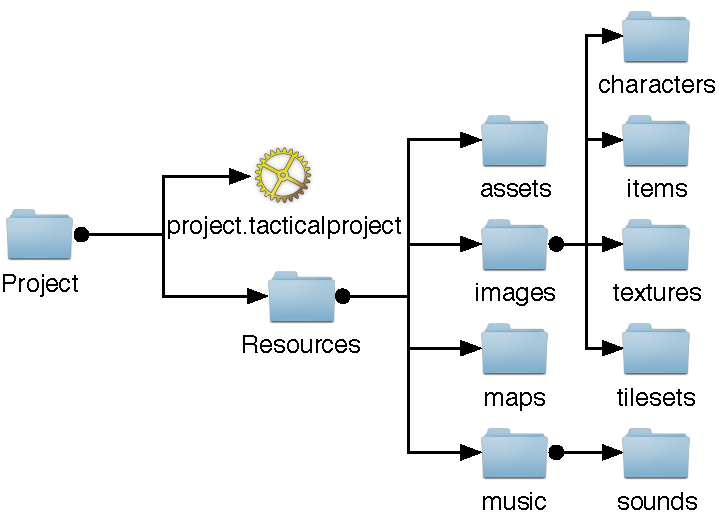
\includegraphics[height=3in]{figures/project.pdf}
	\caption{Editor Project Structure}
	\label{fig:figures_project}
\end{figure}

The main change is the addition of the \texttt{project.tacticalproject} file which contains settings specific to the editor. It also has the added benefit of allowing the user to click on the \texttt{project.tacticalproject} to open the editor if using the Mac version.

\subsubsection{Dialog Data Format}
\label{ssub:dialog_data_format}

The dialog format is actually YAML\cite{yaml}. This allows more formatting options as well the simple format discussed previously. The advantage of using YAML is that there are parsers available for java\cite{snake}. This saved development time since I did not have to build a parser. The main advantage of YAML is that there are very few characters that need to be escaped namely \textbf{:} if it appears at the start of the dialog's text or speaker's name. \textbf{\#} also has to be escaped since it is the comment character in \texttt{YAML}. Since these characters are fairly uncommon in dialog, it should not pose too much inconvenience to the user. In any case the use  of the form \texttt{- Speaker: |-}, then  writing the text on an intended line escapes all characters in the block, solving this problem.

\begin{lstlisting}[caption=A example show the features of the dialog's data format]
- Speaker:   Some text.
- none:      no speaker.
- New Enemy 2: |-
    "All the text in this block (until two newlines),
    are part of New Enemy 2's dialog". 
    No characters need to be escaped in this block e.g #  : \

- Other speaker: Even more text.
\end{lstlisting}
Specifically the dialog must satisfy the following:
\begin{itemize}
	\item  At least one portion of text. A empty file is invalid
	\item  Each portion of text must have a speaker identified by their name or \texttt{none} for no speaker.
	\item  No other elements are allowed.
\end{itemize}

When the dialog is imported, if there is a unit with  the specified name, it is associated with the  portion of text otherwise the text is treated as having no speaker.


\subsection{Data Format Extension Mechanism}
\label{sub:data_format_extension_mechanism}

The user can use their own code to further customise the engine. This section will describe the steps the user needs to take by using the \texttt{Around} weapon as example. This class was originally implemented using the extension mechanism before moving it to the engine. 

To uses their own code the user first has implement the required interface e.g \texttt{IWeapon} for making a custom weapon.  For weapons (as well as skills) there are convenient classes namely (\texttt{AbstractWeapon} and \texttt{AbstractSkill}) which provides methods for bound checking and generating a diamond of the specified size around the specified tile. 

Using \texttt{AbstractWeapon} there only one required method to be implemented, namely \texttt{getAttackRange} which specify which tiles are reachable. For the \texttt{Around} weapon the attack range is the 8 tiles around the attacker. Users can also override the \texttt{getTargets} method to allow multiple targets, in \texttt{Around}'s case it attack \emph{any} unit(including allied units) on any of the 8 tiles.  The \texttt{boundcheck} method which removes any invalid locations from a \texttt{Collection} can be optionally used, to save the user from having to figure out if the tiles would valid\footnote{Especially important since there are a lot of edge cases such as empty tiles, immovable tiles and units occupying a tile.}

One other requirement is that the custom class must be in a package (e.g custom.Around). To use the weapon in a game add the follow entry to the \texttt{Resources/assets/weapons.xml} file of a project.

\begin{lstlisting}[caption=Example of a custom weapon]
<entry>
  <uuid>3e07fa06-184b-41a1-9d2a-5ae87d97f012</uuid>
  <custom.Around uuid="3e07fa06-184b-41a1-9d2a-5ae87d97f012">
    <name>Ball</name>
    <strength>4</strength>
    <range>1</range>
    <imageRef>10-1</imageRef>
  </custom.Around>
</entry>
\end{lstlisting}

As shown above the full qualified classname is used in the above xml. This is used to dynamically load the class. The fields for the class can also be specified in the weapon's tag.  The class then has to be packaged inside a \texttt{jar} and put of the \texttt{classpath} when running the game. For the Mac OS X application it is simpler, requiring the user to place the jar in \lstinline{bundle/Tactical.app/Contents/Resources/Java} and add \texttt{:\$JAVAROOT/WeaponJarName.jar} to end of the \texttt{ClassPath} key in   \lstinline{bundle/Tactical.app/Contents/Info.plist}. This allows the Mac application to still work without any external dependencies.

%TODO Data Format Extension Mechanism
